%!TEX root = ./template-skripsi.tex
%-------------------------------------------------------------------------------
%                            	BAB IV
%               		KESIMPULAN DAN SARAN
%-------------------------------------------------------------------------------

\chapter{HASIL DAN PEMBAHASAN}

\section{Implementasi}

\subsection{Hasil Crawling}

Dalam penelitian ini, situs yang digunakan adalah \textit{thehill.com} 
karena artikel dari situs tersebut menyediakan \textit{tag} di dalam 
artikel. Selain itu, adanya variasi \textit{tag} di dalam situs 
tersebut juga menjadi alasan menggunakan situs ini sebagai bahan 
untuk penelitian.

% GAMBAR THEHILL.COM
\begin{figure}[H]
  \centering
  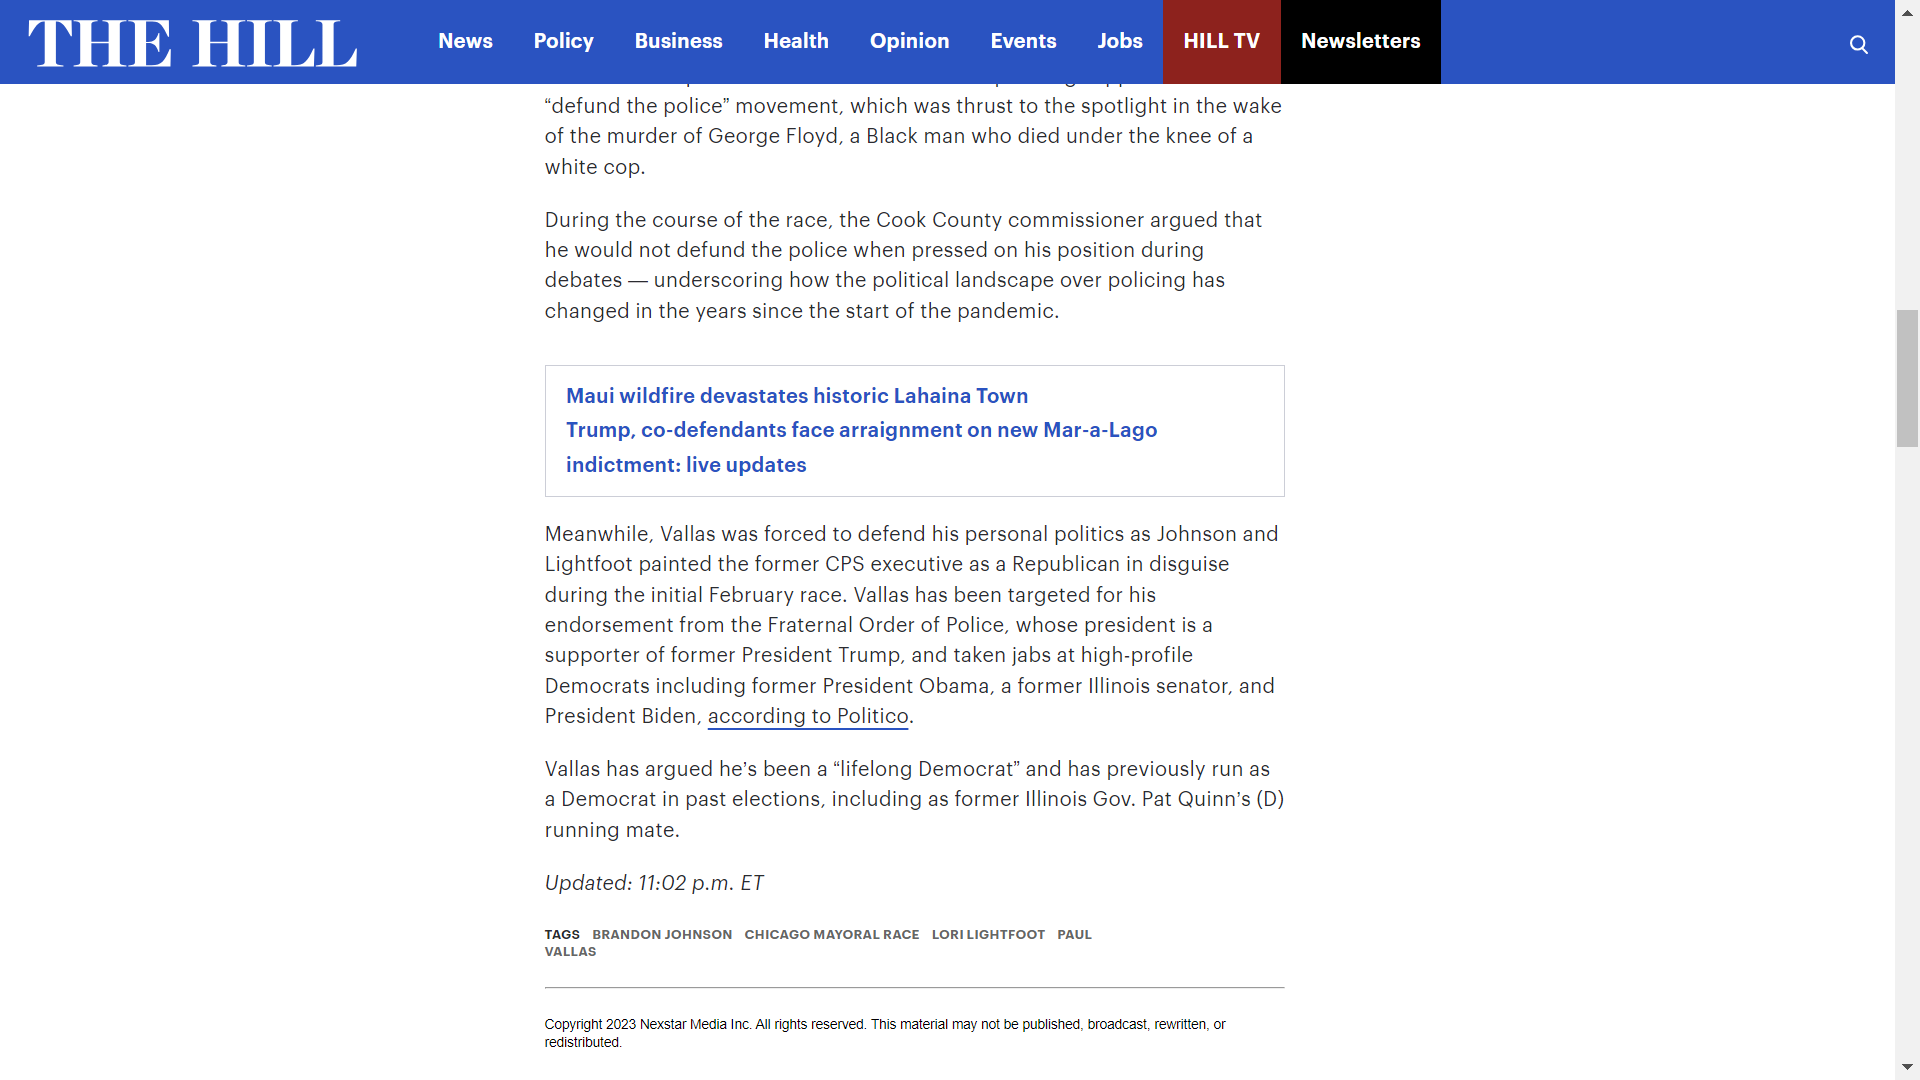
\includegraphics[width=0.75\textwidth]{gambar/bab_4_image/the-hill.png}
  \caption{Contoh \textit{tag} dari artikel thehill.com}
  \label{gambar:thehill}
\end{figure}

Untuk mendapatkan data-data seperti itu, penulis menggunakan 
\textit{crawler}. Dalam \emph{table} "\emph{page\_informations}", kolom yang dipakai 
nantinya adalah kolom \textit{id\_page}, \textit{content\_article}, 
dan \textit{title}. Kemudian, di dalam \textit{page\_tags}, 
kolom yang digunakan adalah kolom \textit{tag} dan \textit{page\_id}.  

% GAMBAR DATASET
\begin{figure}[H]
  \centering
  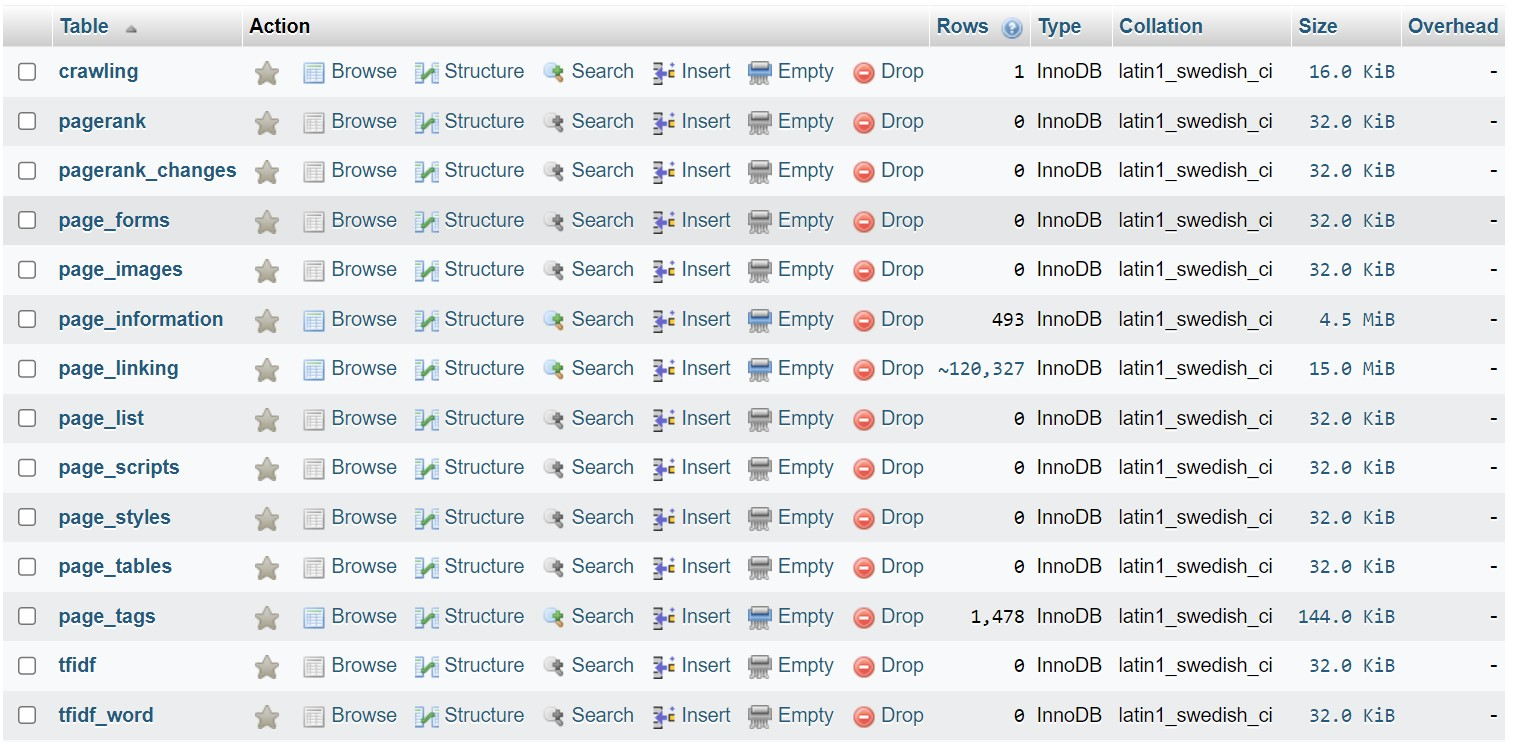
\includegraphics[width=0.75\textwidth]{gambar/bab_4_image/dataset.jpg}
  \caption{Dataset yang digunakan}
  \label{gambar:dataset}
\end{figure}

% GAMBAR DATASET TABLE PAGE tags
\begin{figure}[H]
  \centering
  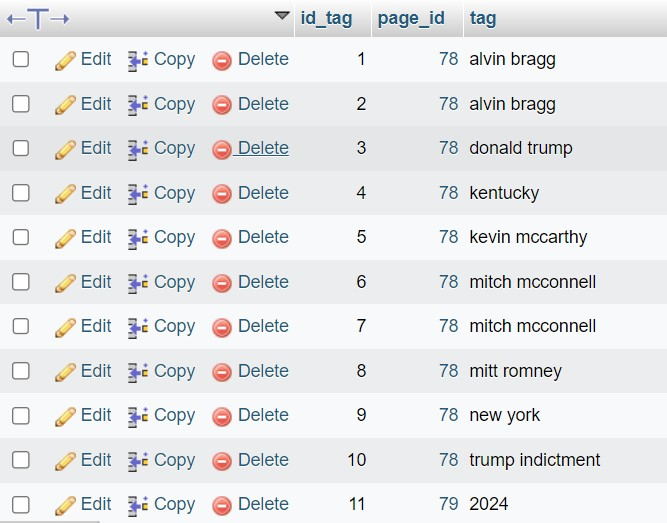
\includegraphics[width=1\textwidth]{gambar/bab_4_image/dataset tag.jpg}
  \caption{Dataset pada tabel \textit{page\_tags}}
  \label{gambar:datasetTag}
\end{figure}

% GAMBAR DATASET TABLE PAGE INFORMATION
\begin{figure}[H]
  \centering
  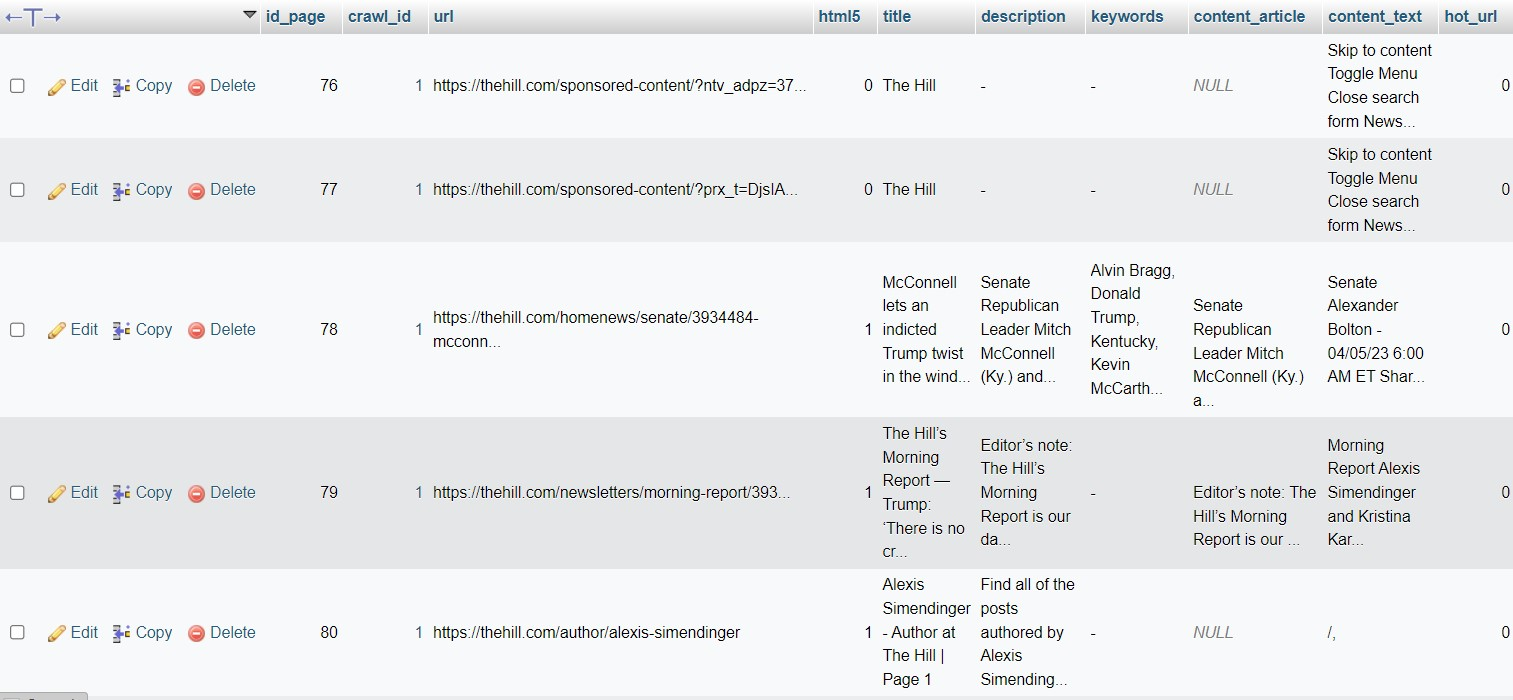
\includegraphics[width=1\textwidth]{gambar/bab_4_image/dataset article.jpg}
  \caption{Dataset pada tabel \textit{page\_informations}}
  \label{gambar:datasetInformation}
\end{figure}

\subsection{Pengambilan Data dari Database}

Data-data yang diambil adalah \emph{tag}, \emph{id} dari artikel, 
judul artikel, dan isi artikel melalui fungsi \emph{get\_data} 
pada \emph{file} \emph{data\_from\_database.py}.

% GAMBAR DARI HASIL PENGAMBILAN DATABASE

\begin{figure}[H]
  \centering
  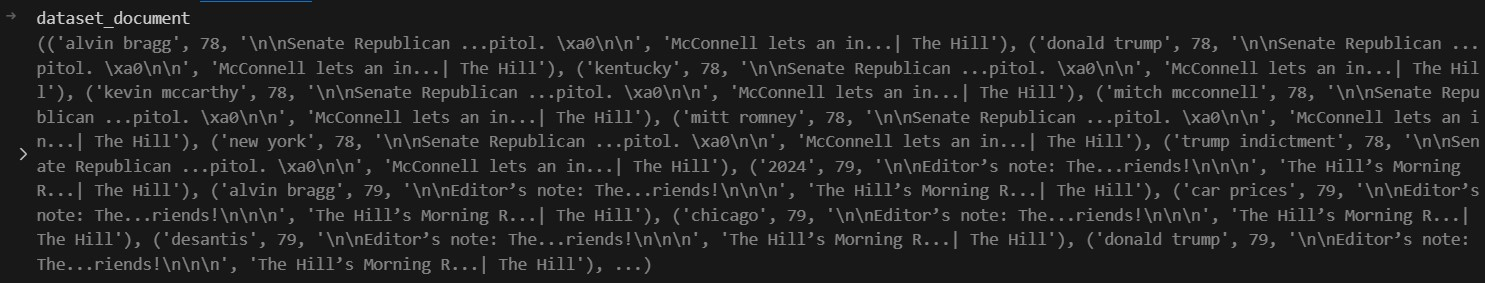
\includegraphics[width=1\textwidth]{gambar/bab_4_image/pengambilan data.jpg}
  \caption{Dataset yang digunakan}
  \label{gambar:pengambilanData}
\end{figure}

\subsection{Penginputan}

Untuk inputnya, $D$ didapat dari \textit{id} dan judul dari artikel yang ada. 
$T$ didapat dari \textit{tag} yang telah dikumpulkan. 
Lalu, $S$ didapat dari kata yang unik dari isi-isi artikel.
Selanjutnya, $K$ bernilai 2, $M$ bernilai 2, dan $L$ bernilai 2. 

\subsection{Mengolah Data Menjadi Matriks}

Data-data tersebut nantinya akan diolah menjadi matriks berdasarkan persamaan (\ref{w_ab}) 
yang di mana matriks $A$ adalah relasi antara \emph{tag} dengan dokumen dan 
matriks $B$ adalah relasi antara dokumen dengan \emph{word}. 
Untuk melakukan proses ini, diperlukan fungsi \emph{document\_processing} 
pada \textit{file} \textit{input\_processing.py}.

% GAMBAR HASIL OUTPUT DARI MATRIX A dan B
\begin{figure}[H]
  \centering
  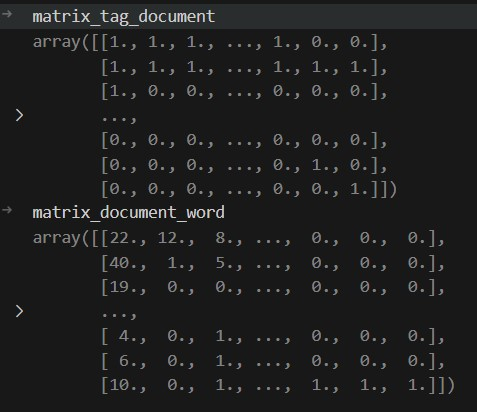
\includegraphics[width=0.75\textwidth]{gambar/bab_4_image/matrix tag document dan matrix document word.jpg}
  \caption{Matrix Tag Document dan Matrix Document Word}
  \label{gambar:matrixTagDocument}
\end{figure}

Lalu, kedua matriks tersebut disatukan hingga menjadi matriks $W$ 
berdasarkan persamaan (\ref{w_ab}) denggan menggunakan fungsi 
\textit{matrixABtoW} pada \textit{file} \textit{matrix\_processing.py}.

% GAMBAR HASIL OUTPUT MATRIX W
\begin{figure}[H]
  \centering
  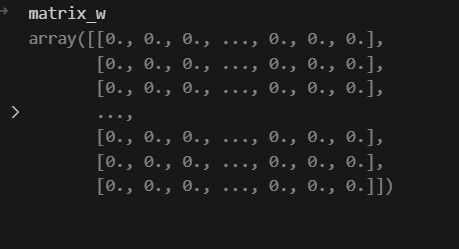
\includegraphics[width=0.75\textwidth]{gambar/bab_4_image/matrix w.jpg}
  \caption{Matrix W}
  \label{gambar:matrixW}
\end{figure}

\subsection{Menghitung Low Rank Approximation Matrix Menggunakan Algoritma Lanczos}

Untuk merubah matriks $W$ menjadi matriks $\tilde{W}$, diperlukan matriks
$Q_k$ dan $T_k$. Algoritma \textit{Lanczos Iteration} dapat digunakan untuk
mencari nilai dari matriks tersebut.

Dalam mencari nilai matriks $Q_k$ dan $T_k$, diperlukan \textit{function} 
\textit{lanczos\_iteration} pada \textit{file} \textit{low\_rank\_approximation\_matrix.py}.
Hasilnya adalah sebagai berikut.


% GAMBAR HASIL OUTPUT MATRIX Q DAN T
\begin{figure}[H]
  \centering
  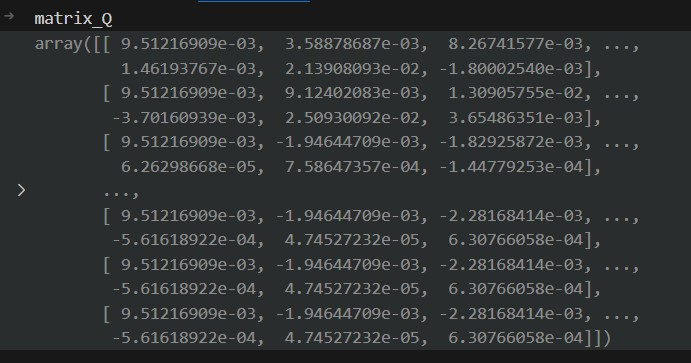
\includegraphics[width=0.75\textwidth]{gambar/bab_4_image/Matrix q.jpg}
  \caption{Matriks $Q$}
  \label{gambar:matrixQ}
\end{figure}

\begin{figure}[H]
  \centering
  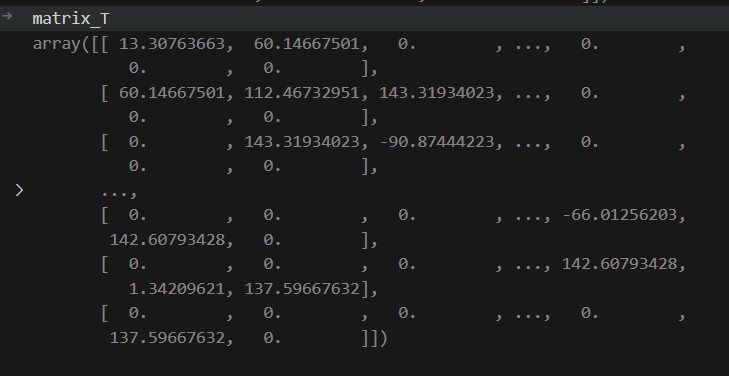
\includegraphics[width=0.75\textwidth]{gambar/bab_4_image/Matrix t.jpg}
  \caption{Matriks $T$}
  \label{gambar:matrixT}
\end{figure}

Selanjutnya, mencari nilai dari matriks $\tilde{W}$ dengan menggunakan \textit{function}
\textit{low\_rank\_approximation\_matrix} pada \textit{file} \textit{low\_rank\_approximation\_matrix.py}.
Hasilnya bisa dilihat di bawah ini.
% GAMBAR HASIL OUTPUT MATRIX W_hat

\begin{figure}[H]
  \centering
  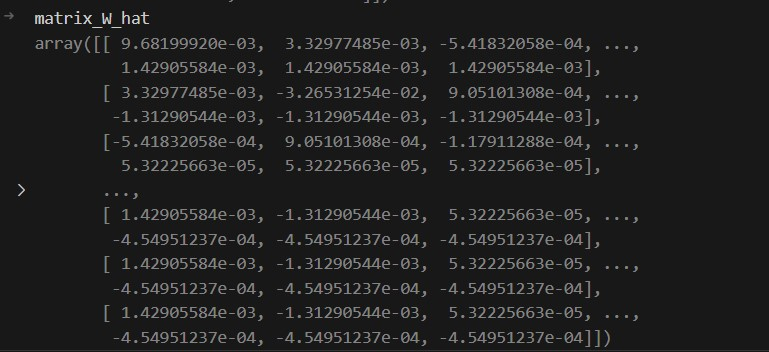
\includegraphics[width=0.75\textwidth]{gambar/bab_4_image/matrix w hat.jpg}
  \caption{Matriks $\tilde{W}$}
  \label{gambar:matrixWHat}
\end{figure}

\subsection{Melakukan Partisi W ke dalam Klaster K}

Agar dapat melakukan \textit{Bipartite Graph Partition}, perlu algoritma 
bernama \textit{Spectral Recursive Embedding}. Hasil dari partisi ini adalah
membentuk dua \textit{graph} terbaru dalam bentuk matriks. Untuk partisinya,
ditentukan oleh banyaknya $K$ yang telah diatur. Partisi ini menggunakan
fungsi \textit{spectral\_recursive\_embedding} pada \textit{file} 
\textit{spectral\_recursive\_embedding.py}.

% GAMBAR HASIL OUTPUT MATRIKS PARTITION
\begin{figure}[H]
  \centering
  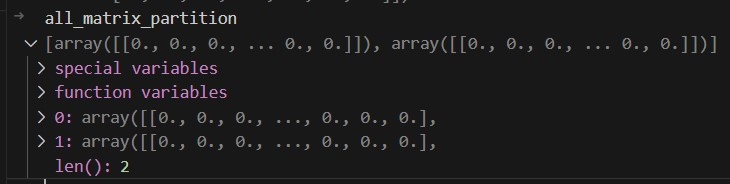
\includegraphics[width=1\textwidth]{gambar/bab_4_image/matrix partisi.jpg}
  \caption{Matriks hasil partisi}
  \label{gambar:matriksPartisi}
\end{figure}

\subsection{Melakukan Pelabelan Setiap Dokumen}

Setiap dokumen dilabelkan berdasarkan hasil partisi yang telah dilakukan.
Pelabelan ini tergantung banyaknya klaster yang disediakan. Jika terdiri
dari dua klaster, berarti dokumen tersebut akan dimasukkan ke dalam klaster
pertama atau klaster kedua sesuai hasil dari \textit{Bipartite Graph Partition} dengan
menggunakan fungsi \textit{assign\_label\_cluster} pada \textit{file}
\textit{assign\_label.py}.

% GAMBAR HASIL PELABELAN DOKUMEN
\begin{figure}[H]
  \centering
  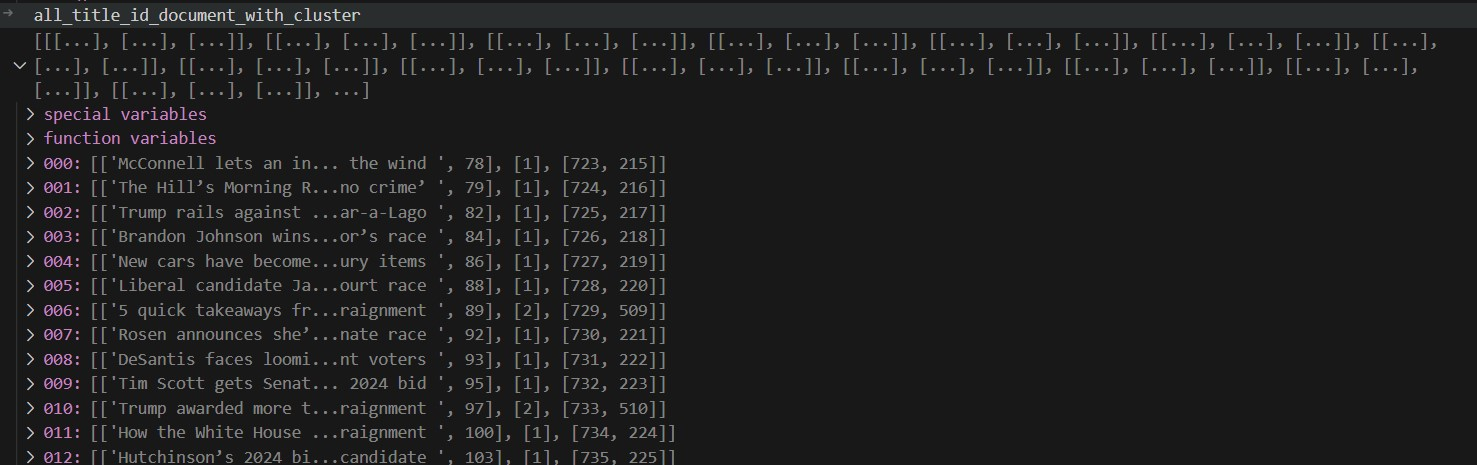
\includegraphics[width=1\textwidth]{gambar/bab_4_image/pelabelan dokumen.jpg}
  \caption{Pelabelan dokumen}
  \label{gambar:pelabelanDokumen}
\end{figure}

Pada variabel \textit{all\_title\_id\_document\_with\_cluster}, terdapat beberapa data di setiap \textit{index}.
Data tersebut yaitu
\begin{enumerate}
  \item Judul dokumen dan \textit{id}.
  \item Label klaster.
  \item \textit{Node} keberapa dalam suatu \textit{bipartite graph}.
\end{enumerate}

\subsection{Menghitung Rank(T) untuk setiap Tag}

Setiap \textit{tag} yang ada di dataset, perlu dihitung terlebih dahulu nilai
\textit{Rank(T)}. Untuk menghitung \textit{Rank(T)}, akan menggunakan fungsi
\textit{node\_rankt} dalam \textit{file} \textit{node\_rank\_t.py}. Hasilnya
sebagai berikut.

% GAMBAR RANK T

\begin{figure}[H]
  \centering
  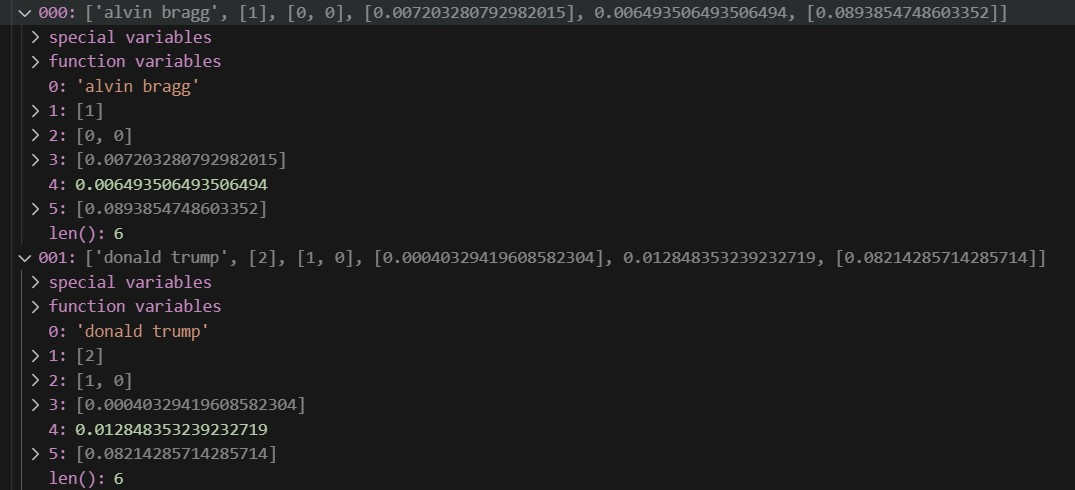
\includegraphics[width=1\textwidth]{gambar/bab_4_image/Node Rank T.jpg}
  \caption{Rank(T)}
  \label{gambar:rankT}
\end{figure}

Dari hasil ini, terdapat dua \textit{tag} yang digunakan sebagai contoh yaitu 
\textit{Alvin Bragg} dan \textit{Donald Trump}. \textit{Alvin Bragg} memiliki nilai 
\textit{N Precision} sebesar 0,893855 , \textit{N Recall} sebesar 0,006494, dan
\textit{Rank(T)} sebesar 0,007203. 

\subsection{Membuat Two Way Poisson Mixture Model}

Dalam membuat \textit{Two Way Poisson Mixture Model}, terdapat beberapa hal yang
diperlukan yaitu relasi antara dokumen dengan \textit{word vocabulary},
banyaknya komponen $M$, banyaknya klaster $K$, dan banyaknya 
\textit{word cluster} $L$.

Awalnya, perlu mencari $\pi_{m}$ dengan cara menghitung seluruh dokumen dalam komponen $m$
dibagi dengan seluruh dokumen yang ada menggunakan fungsi 
\textit{first\_prior\_probability} pada \textit{file} \textit{two\_way\_poisson\_mixture\_model.py}. 
Dengan menggunakan banyaknya komponen $M$ berjumlah dua, menghasilkan hasil sebagai berikut.

\begin{figure}[H]
  \centering
  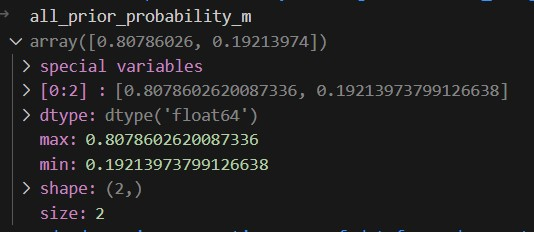
\includegraphics[width=0.75\textwidth]{gambar/bab_4_image/all_prior_probability_m.jpg}
  \caption{ $\pi_{m}$ }
  \label{gambar:priorProbability}
\end{figure}

Selanjutnya, mencari nilai $\tilde{\lambda_{m}}$ untuk setiap kata. Nilai $\tilde{\lambda_{m}}$
untuk setiap kata didapat dari nilai rata-rata kemunculan kata tersebut di setiap dokumen $d$
dalam setiap komponen $m$. Dengan menggunakan fungsi \textit{lambda\_m\_j\_list} pada \textit{file}
\textit{two\_way\_poisson\_mixture\_model.py} hasilnya sebagai berikut.

\begin{figure}[H]
  \centering
  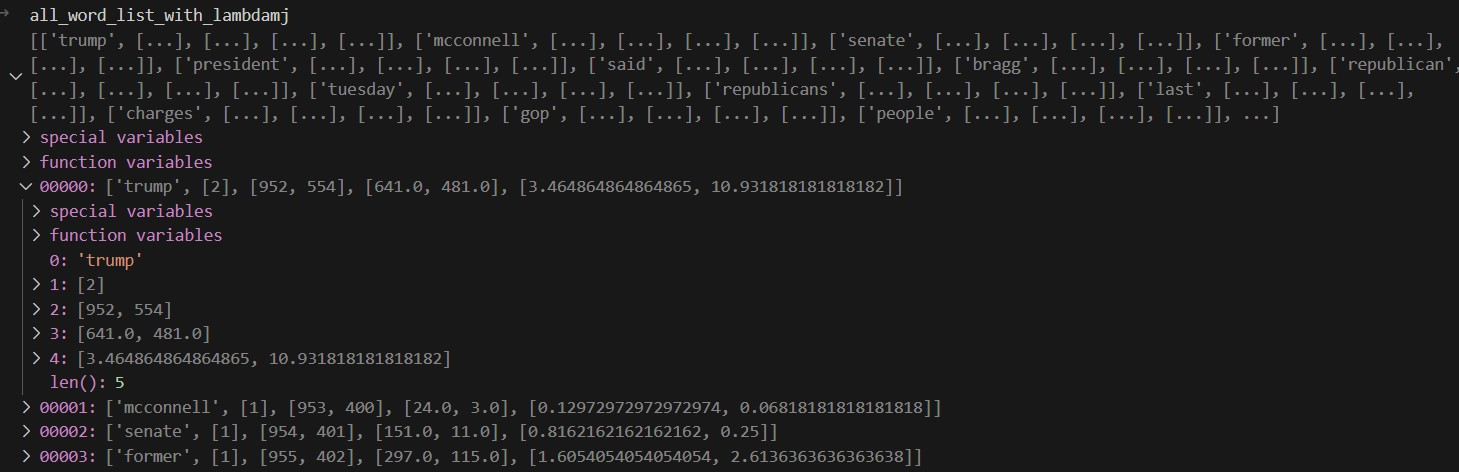
\includegraphics[width=1\textwidth]{gambar/bab_4_image/all word list lamda mj.jpg}
  \caption{ Daftar kata dengan nilai $\tilde{\lambda_{m}}$}
  \label{gambar:wordListLambdaMJ}
\end{figure}

Kemudian, mencari nilai $p_{i,m}$ dalam setiap dokumen untuk memulai fase \textit{E-step}  
dengan menggunakan fungsi \textit{p\_im\_list} pada \textit{file}
\textit{two\_way\_poisson\_mixture\_model.py}. Hasil yang didapat sebagai berikut.

\begin{figure}[H]
  \centering
  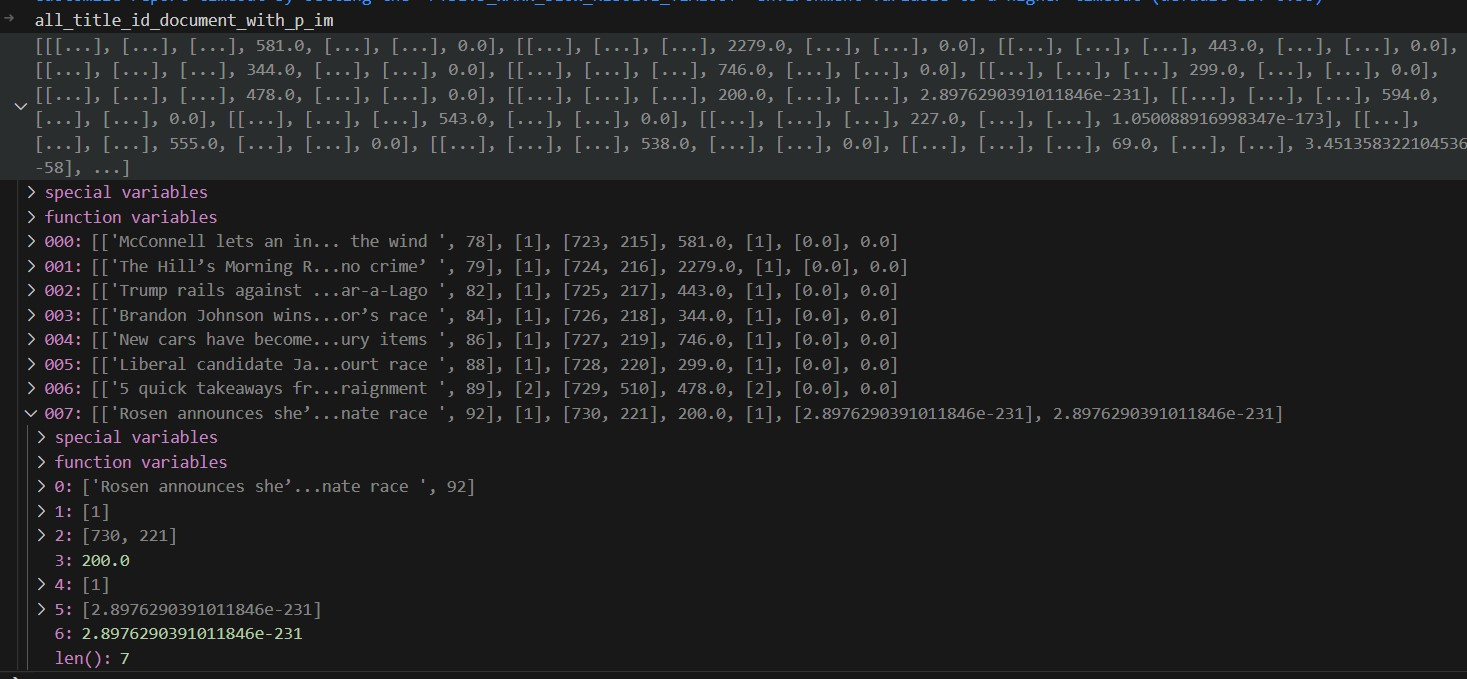
\includegraphics[width=0.75\textwidth]{gambar/bab_4_image/pim in document.jpg}
  \caption{Nilai $p_{i,m}$ pada setiap dokumen }
  \label{gambar:pim}
\end{figure}

Setiap \textit{index} dari variabel tersebut mengandung beberapa nilai yaitu
\begin{enumerate}
  \item Nilai dari judul dokumen dan \textit{id} dokumen.
  \item Klaster $k$ dari dokumen tersebut.
  \item \textit{Node} keberapa dari suatu \textit{bipartite graph} awal dan \textit{bipartite graph} setelah partisi.
  \item Banyaknya kata dalam dokumen.
  \item Komponen $m$ dari dokumen tersebut.
  \item Nilai dari $p_{i,m}$.
  \item Nilai dari $P(D=d|K=k)$ dari dokumen.
\end{enumerate}

Dari data di atas, nilai $p_{i,m}$ sangat rendah dan beberapa diantaranya 0. Hal ini dikarenakan perhitungan \textit{product}
dari nilai $\theta$ yang rendah, tapi nilai $p$ (banyaknya kata unik) yang banyak dalam persamaan \ref*{e_step}.

Selanjutnya adalah melakukan \textit{M-step}. Dalam penelitian ini, iterasi yang digunakan yaitu lima kali.

\subsection{Rekomendasi Tag}

Fungsi utama dari algoritma ini adalah membuat rekomendasi \textit{tag} berdasarkan
data latih yang tersedia. Saat ini, algoritma tersebut mampu memberikan sepuluh
pilihan \textit{tag} sesuai hasil rekomendasi. Dengan menggunakan fungsi
\textit{tag\_recommendation\_mass} pada \textit{file} \textit{tag\_recommendation\_for\_new\_document.py},
hasil yang didapat sebagai berikut.

% GAMBAR SALAH SATU CONTOH HASIL REKOMENDASI
\begin{figure}[H]
  \centering
  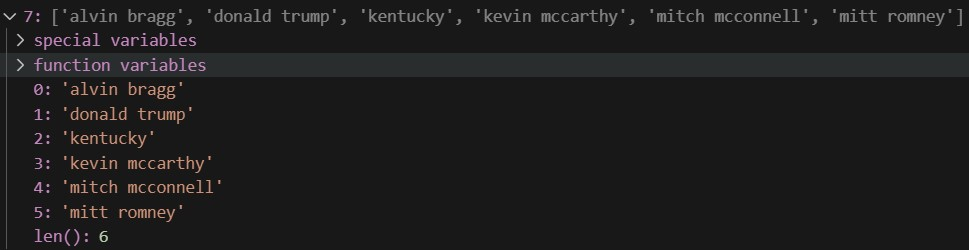
\includegraphics[width=1\textwidth]{gambar/bab_4_image/rekomendasi tag.jpg}
  \caption{Contoh dari hasil rekomendasi \textit{Tag}}
  \label{gambar:rekomendasiTag}
\end{figure}

\section{Hasil Pengujian}

Berdasarkan hasil pengujian, akurasi dari rekomendasi \textit{tag} 
dengan menggunakan algoritma \textit{Bipartite Graph Partition}
dan \textit{Two Way Poisson Mixture Model} adalah sebagai berikut.

% GAMBAR HASIL PENGUJIAN

\begin{figure}[H]
  \centering
  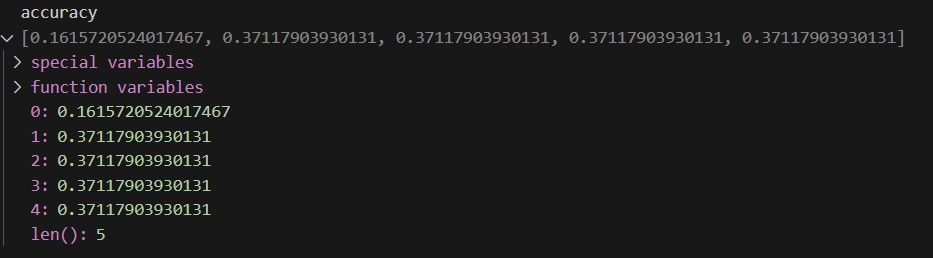
\includegraphics[width=1\textwidth]{gambar/bab_4_image/Akurasi.jpg}
  \caption{Contoh dari hasil rekomendasi \textit{Tag}}
  \label{gambar:akurasi}
\end{figure}

Saat melakukan iterasi di \textit{Poisson Mixture Model} sebanyak lima kali,
akurasi tertinggi sebanyak 37\% dengan jumlah data 229 dokumen dan 723 \textit{tag}.

Untuk pengujian ini, tidak menggunakan data uji dan justru melakukan pengujian dengan data yang sama
seperti data latih. 

\section{Hasil Analisa}

Berdasarkan hasil pengujian, jumlah akurasi terbilang sedikit yaitu 37,118\%. Tentunya, terdapat
beberapa faktor kenapa hasilnya rendah yaitu

\begin{enumerate}
  \item Penggunaan $K$ yang sangat sedikit saat melakukan \textit{Bipartite Graph Partition}.
  \item Nilai $P(D = d|K = k)$ yang terlalu sedikit juga menentukan rendahnya akurasi.
  \item Adanya kemungkinan hasil kodingan program yang kurang baik.
\end{enumerate}

Salah satu penyebabnya adalah saat perhitungan dengan menggunakan persamaan \ref*{e_step}. Dalam
melakukan perhitungan ini, nilai rata-rata pada $\theta \left(d(i, j) \mid \tilde{\lambda}_{m, i, j}^{(t)}\right)$
adalah sebagai berikut.

\begin{figure}[H]
  \centering
  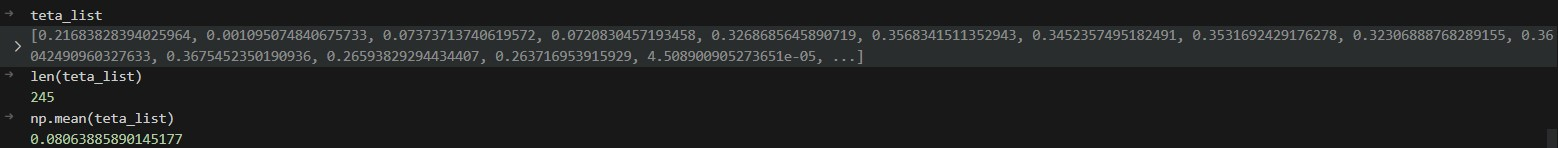
\includegraphics[width=1\textwidth]{gambar/bab_4_image/teta_list.jpg}
  \caption{Nilai $\theta \left(d(i, j) \mid \tilde{\lambda}_{m, i, j}^{(t)}\right)$}
  \label{gambar:teta_list}
\end{figure}

Selain itu, kelemahan kodingan program yang telah penulis buat adalah tidak bisa membagi \textit{Bipartite Graph Partition}
sesuai dengan sumber aslinya. Jika program yang penulis buat mampu membagi \textit{Bipartite Graph Partition} sesuai dengan
$K$ yang diinginkan, akurasinya bisa saja meningkat.


% - Hasil-hasil teta yang rendah
% - Tidak tersedianya bipartite graph partition jika K >= 2

% Spesifikasi Laptop yang digunakan.
% Implementasi code.
% Hasil berupa (database, dan isi database. peta graph).